% !TeX TXS-program:compile = txs:///arara
% arara: lualatex: {shell: no, synctex: yes, interaction: batchmode}
% arara: pythontex: {rerun: modified} if found('pytxcode', 'PYTHONTEX#py')
% arara: lualatex: {shell: no, synctex: yes, interaction: batchmode} if found('pytxcode', 'PYTHONTEX#py')
% arara: lualatex: {shell: no, synctex: yes, interaction: batchmode} if found('log', '(undefined references|Please rerun|Rerun to get)')

\documentclass[a4paper,11pt]{article}
\usepackage[]{cp-base}

%tableaux
\usepackage{booktabs}
\setlength\aboverulesep{0.65ex}
\setlength\belowrulesep{0.65ex}
\arrayrulecolor{titrebleu}

%variables
\graphicspath{{./graphics/}}
\donnees[classe={1\up{ère} 2M2},matiere={[SPÉ.MATHS]},mois=Avril,annee=2022,typedoc=QCM,numdoc=2]
%formatage
\author{Pierquet}
\title{\nomfichier}
\hypersetup{pdfauthor={Pierquet},pdftitle={\nomfichier},allbordercolors=white,pdfborder=0 0 0,pdfstartview=FitH}
%divers
\lhead{\entete{\matiere}}
\chead{\entete{\lycee}}
\rhead{\entete{\classe{} - \mois{} \annee}}
\lfoot{\pied{\matiere}}
\cfoot{\logolycee}
\rfoot{\pied{\numeropagetot}}

%commandes pdfform
\renewcommand\LayoutCheckField[2]{#2~~#1}
\newcommand\choix[2]{%
	\raisebox{-.15\baselineskip}{\CheckBox[name=#1#2,width=1em,height=1em,bordercolor=black]{}}%
}
\newcommand\reponse[2]{%
	\raisebox{-.15\baselineskip}{\CheckBox[checkboxsymbol=\ding{95},color=red,name=#1#2,width=1em,height=1em,bordercolor=white]{}}%
}

\begin{document}

\thispagestyle{fancy}

\begin{pycode}
def qcmalea(a,b,c,d):
	from random import shuffle
	reponses = [a,b,c,d]
	shuffle(reponses)
	return reponses

def qcmalea3(a,b,c):
	from random import shuffle
	reponses = [a,b,c]
	shuffle(reponses)
	return reponses

#Question1 - A
ENONCEQ1 = r"Soient A et B deux évènements tels que $P(A)=0,6$ ; $P(B)=0,7$ et $P(A \cup B)=0,95$.\\ Alors $P(A \cap B)$ vaut :"
Q1A = r"\reponse{R1}{A}\choix{Q1}{A}~"
Q1B = r"\reponse{R1}{B}\choix{Q1}{B}~"
Q1C = r"\reponse{R1}{C}\choix{Q1}{C}~"
Q1D = r"\reponse{R1}{D}\choix{Q1}{D}~"
Q1A += r"$0,35$" #OK
Q1B += r"$0,42$"
Q1C += r"$1,3$"
Q1D += r"$0,05$"
reponsesQ1 = qcmalea(Q1A,Q1B,Q1C,Q1D)

#Question2 - A
ENONCEQ2 = r"On a $P\left(A \cap \overline{B}\right)=$"
Q2A = r"\reponse{R2}{A}\choix{Q2}{A}~"
Q2B = r"\reponse{R2}{B}\choix{Q2}{B}~"
Q2C = r"\reponse{R2}{C}\choix{Q2}{C}~"
Q2D = r"\reponse{R2}{D}\choix{Q2}{D}~"
Q2A += r"$0,3$" #OK
Q2B += r"$0,6$"
Q2C += r"$1,06$"
Q2D += r"$0,28$"
reponsesQ2 = qcmalea(Q2A,Q2B,Q2C,Q2D)

#Question3 - A
ENONCEQ3 = r"On a $P_B \left(\overline{A}\right)=$"
Q3A = r"\reponse{R3}{A}\choix{Q3}{A}~"
Q3B = r"\reponse{R3}{B}\choix{Q3}{B}~"
Q3C = r"\reponse{R3}{C}\choix{Q3}{C}~"
Q3D = r"\reponse{R3}{D}\choix{Q3}{D}~"
Q3A += r"$\dfrac{6}{11}$" #OK
Q3B += r"$\dfrac{5}{11}$"
Q3C += r"$0,5\vphantom{\dfrac63}$"
Q3D += r"$0,24\vphantom{\dfrac63}$"
reponsesQ3 = qcmalea(Q3A,Q3B,Q3C,Q3D)

#Question4 - A
ENONCEQ4 = r"On a $P_{\overline{F}}(R)=$"
Q4A = r"\reponse{R4}{A}\choix{Q4}{A}~"
Q4B = r"\reponse{R4}{B}\choix{Q4}{B}~"
Q4C = r"\reponse{R4}{C}\choix{Q4}{C}~"
Q4D = r"\reponse{R4}{D}\choix{Q4}{D}~"
Q4A += r"$0,2\vphantom{\dfrac13}$" #OK
Q4B += r"$0,08\vphantom{\dfrac13}$"
Q4C += r"$\dfrac13$"
Q4D += r"$0,65\vphantom{\dfrac13}$"
reponsesQ4 = qcmalea(Q4A,Q4B,Q4C,Q4D)

#Question5 - A
ENONCEQ5 = r"On a $P\left(F \cap \overline{R}\right)=$"
Q5A = r"\reponse{R5}{A}\choix{Q5}{A}~"
Q5B = r"\reponse{R5}{B}\choix{Q5}{B}~"
Q5C = r"\reponse{R5}{C}\choix{Q5}{C}~"
Q5D = r"\reponse{R5}{D}\choix{Q5}{D}~"
Q5A += r"$0,39\vphantom{\dfrac73}$" #OK
Q5B += r"$0,65\vphantom{\dfrac73}$"
Q5C += r"$0,95\vphantom{\dfrac73}$"
Q5D += r"$\dfrac{7}{12}$"
reponsesQ5 = qcmalea(Q5A,Q5B,Q5C,Q5D)

#Question6 - A
ENONCEQ6 = r"La probabilité de l'évènement $R$ est :"
Q6A = r"\reponse{R6}{A}\choix{Q6}{A}~"
Q6B = r"\reponse{R6}{B}\choix{Q6}{B}~"
Q6C = r"\reponse{R6}{C}\choix{Q6}{C}~"
Q6D = r"\reponse{R6}{D}\choix{Q6}{D}~"
Q6A += r"$0,29$" #OK
Q6B += r"$0,55$"
Q6C += r"$0,07$"
Q6D += r"$0,57$"
reponsesQ6 = qcmalea(Q6A,Q6B,Q6C,Q6D)

#Question7 - A
ENONCEQ7 = r"La probabilité $P_R(F)$ vaut :"
Q7A = r"\reponse{R7}{A}\choix{Q7}{A}~"
Q7B = r"\reponse{R7}{B}\choix{Q7}{B}~"
Q7C = r"\reponse{R7}{C}\choix{Q7}{C}~"
Q7D = r"\reponse{R7}{D}\choix{Q7}{D}~"
Q7A += r"$\dfrac{21}{29}$" #OK
Q7B += r"$0,35\vphantom{\dfrac23}$"
Q7C += r"$0,95\vphantom{\dfrac23}$"
Q7D += r"$\dfrac{7}{11}$"
reponsesQ7 = qcmalea(Q7A,Q7B,Q7C,Q7D)

#Question8 - A
ENONCEQ8 = r"Soient $D$ et $K$ deux évènements indépendants tels que $P(D)=0,31$ et $P(K)=0,53$.\\ Alors la probabilité de l'évènement $D \cap K$ vaut :"
Q8A = r"\reponse{R8}{A}\choix{Q8}{A}~"
Q8B = r"\reponse{R8}{B}\choix{Q8}{B}~"
Q8C = r"\reponse{R8}{C}\choix{Q8}{C}~"
Q8D = r"\reponse{R8}{D}\choix{Q8}{D}~"
Q8A += r"$0,1643\vphantom{\dfrac33}$" #OK
Q8B += r"$\dfrac{31}{53}$"
Q8C += r"$0,84\vphantom{\dfrac33}$"
Q8D += r"$0,22\vphantom{\dfrac33}$"
reponsesQ8 = qcmalea(Q8A,Q8B,Q8C,Q8D)

#Question9 - A
ENONCEQ9 = r"Soient $G$ et $H$ deux évènements indépendants tels que $P(G)=0,7$ et $P(\overline{H})=0,4$. Alors $P(G \cup H)=$"
Q9A = r"\reponse{R9}{A}\choix{Q9}{A}~"
Q9B = r"\reponse{R9}{B}\choix{Q9}{B}~"
Q9C = r"\reponse{R9}{C}\choix{Q9}{C}~"
Q9D = r"\reponse{R9}{D}\choix{Q9}{D}~"
Q9A += r"$0,88\vphantom{\dfrac33}$" #OK
Q9B += r"$1,3\vphantom{\dfrac33}$"
Q9C += r"$\dfrac{31}{70}$"
Q9D += r"$0,28\vphantom{\dfrac33}$"
reponsesQ9 = qcmalea(Q9A,Q9B,Q9C,Q9D)

#Question10 - A
ENONCEQ10 = r"On considère la fonction \calgpython{} donnée ci-dessous.\\ Quelle est la probabilité que cette fonction renvoie \cpy{['bleu','rouge']} ?"
Q10A = r"\reponse{R10}{A}\choix{Q10}{A}~"
Q10B = r"\reponse{R10}{B}\choix{Q10}{B}~"
Q10C = r"\reponse{R10}{C}\choix{Q10}{C}~"
Q10D = r"\reponse{R10}{D}\choix{Q10}{D}~"
Q10A += r"$0,05$" #OK
Q10B += r"$0,1\vphantom{\dfrac23}$"
Q10C += r"$\dfrac{23}{38}$"
Q10D += r"$0,7\vphantom{\dfrac23}$"
reponsesQ10 = qcmalea(Q10A,Q10B,Q10C,Q10D)
\end{pycode}

\part*{QCM - Probabilités conditionnelles}

\medskip

\begin{Form}

\textbf{\Large NOM Prénom : }~\raisebox{-.25\baselineskip}{\TextField[value=,width=10cm,height=2em,charsize=14pt,name=nomprenom,bordercolor=black]{}} \hfill~\textbf{\Large Note : }~\raisebox{-.25\baselineskip}{\TextField[width=2em,height=2em,charsize=14pt,name=note,bordercolor=black,color=1 0 0,align=1]{}}

\bigskip

\emph{Cet exercice est un questionnaire à choix multiple. Pour chacune des questions suivantes, \textbf{une seule} des quatre réponses proposées est exacte. Une bonne réponse rapporte un point. Une réponse fausse, une réponse multiple ou l’absence de réponse à une question ne rapporte ni n’enlève de point.\\
Pour répondre, compléter, à l'aide du logiciel {\small \red \textsf{Acrobat Reader} \faIcon[regular]{file-pdf}}.}

\begin{enumerate}
	\item \py{ENONCEQ1}
	\begin{center}
		%\renewcommand{\arraystretch}{1.25}
		\begin{tabularx}{\linewidth}{@{}X@{}X@{}}
			\toprule
			\py{reponsesQ1[0]} & \py{reponsesQ1[1]} \\ \midrule
			\py{reponsesQ1[2]} & \py{reponsesQ1[3]} \\ \bottomrule
		\end{tabularx}
	\end{center}
\end{enumerate}

Pour les questions \ptno{2} et \ptno{3}, on considère le tableau suivant :
\begin{center}
	\renewcommand{\arraystretch}{1.25}
	\arrayrulecolor{darkgray}
	\setlength\arrayrulewidth{1pt}
	{\small \begin{tabularx}{10cm}{|Y|Y|Y|Y|}
		\cline{2-4}
		\multicolumn{1}{c|}{} & \textsf{A} & $\mathsf{\overline{A}}$ & \textsf{Total} \\ \hline
		\textsf{B} & \textsf{100} & \textsf{120} & \textsf{220} \\ \hline
		$\mathsf{\overline{B}}$ & \textsf{150} & \textsf{130} & \textsf{280} \\ \hline
		\textsf{Total} & \textsf{250} & \textsf{250} & \textsf{500} \\ \hline
	\end{tabularx}}
	\arrayrulecolor{titrebleu}
\end{center}

\begin{enumerate}[resume]
	\item \py{ENONCEQ2}
	\begin{center}
		%\renewcommand{\arraystretch}{2.25}
		\begin{tabularx}{\linewidth}{@{}X@{}X@{}}
			\toprule
			\py{reponsesQ2[0]} & \py{reponsesQ2[1]} \\ \midrule
			\py{reponsesQ2[2]} & \py{reponsesQ2[3]} \\ \bottomrule
		\end{tabularx}
	\end{center}
	\item \py{ENONCEQ3}
	\begin{center}
		%\renewcommand{\arraystretch}{1.75}
		\begin{tabularx}{\linewidth}{@{}X@{}X@{}}
			\toprule
			\py{reponsesQ3[0]} & \py{reponsesQ3[1]} \\ \midrule
			\py{reponsesQ3[2]} & \py{reponsesQ3[3]} \\ \bottomrule
		\end{tabularx}
	\end{center}
\end{enumerate}

Pour les \textbf{4} questions suivantes, on considère l'arbre de probabilités suivant :
\begin{center}
	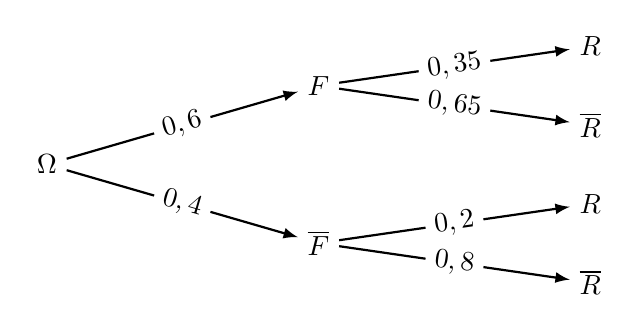
\begin{tikzpicture}[xscale=1,yscale=1]
		\tikzstyle{fleche}=[->,>=latex,thick]
		\tikzstyle{noeud}=[]
		\tikzstyle{feuille}=[]
		\tikzstyle{etiquette}=[midway,sloped,fill=white]
		
		\def\DistanceInterNiveaux{3}
		\def\DistanceInterFeuilles{1}
		
		\def\NiveauA{(0)*\DistanceInterNiveaux}
		\def\NiveauB{(1.15)*\DistanceInterNiveaux}
		\def\NiveauC{(2.3)*\DistanceInterNiveaux}
		\def\InterFeuilles{(-1)*\DistanceInterFeuilles}
		
		\node[noeud] (R) at ({\NiveauA},{(1.5)*\InterFeuilles}) {$\Omega$};
		\node[noeud] (Ra) at ({\NiveauB},{(0.5)*\InterFeuilles}) {$F$};
		\node[feuille] (Raa) at ({\NiveauC},{(0)*\InterFeuilles}) {$R$};
		\node[feuille] (Rab) at ({\NiveauC},{(1)*\InterFeuilles}) {$\overline{R}$};
		\node[noeud] (Rb) at ({\NiveauB},{(2.5)*\InterFeuilles}) {$\overline{F}$};
		\node[feuille] (Rba) at ({\NiveauC},{(2)*\InterFeuilles}) {$R$};
		\node[feuille] (Rbb) at ({\NiveauC},{(3)*\InterFeuilles}) {$\overline{R}$};
		
		\draw[fleche] (R)--(Ra) node[etiquette] {$0,6$};
		\draw[fleche] (Ra)--(Raa) node[etiquette] {$0,35$};
		\draw[fleche] (Ra)--(Rab) node[etiquette] {$0,65$};
		\draw[fleche] (R)--(Rb) node[etiquette] {$0,4$};
		\draw[fleche] (Rb)--(Rba) node[etiquette] {$0,2$};
		\draw[fleche] (Rb)--(Rbb) node[etiquette] {$0,8$};
	\end{tikzpicture}
\end{center}

\begin{enumerate}[resume]
	\item \py{ENONCEQ4}
	\begin{center}
		%\renewcommand{\arraystretch}{1.75}
		\begin{tabularx}{\linewidth}{@{}X@{}X@{}}
			\toprule
			\py{reponsesQ4[0]} & \py{reponsesQ4[1]} \\ \midrule
			\py{reponsesQ4[2]} & \py{reponsesQ4[3]} \\ \bottomrule
		\end{tabularx}
	\end{center}
	\newpage
	\item \py{ENONCEQ5}
	\begin{center}
		%\renewcommand{\arraystretch}{1.75}
		\begin{tabularx}{\linewidth}{@{}X@{}X@{}}
			\toprule
			\py{reponsesQ5[0]} & \py{reponsesQ5[1]} \\ \midrule
			\py{reponsesQ5[2]} & \py{reponsesQ5[3]} \\ \bottomrule
		\end{tabularx}
	\end{center}
	\item \py{ENONCEQ6}
	\begin{center}
		%\renewcommand{\arraystretch}{1.75}
		\begin{tabularx}{\linewidth}{@{}X@{}X@{}}
			\toprule
			\py{reponsesQ6[0]} & \py{reponsesQ6[1]} \\ \midrule
			\py{reponsesQ6[2]} & \py{reponsesQ6[3]} \\ \bottomrule
		\end{tabularx}
	\end{center}
	\item \py{ENONCEQ7}
	\begin{center}
		%\renewcommand{\arraystretch}{1.75}
		\begin{tabularx}{\linewidth}{@{}X@{}X@{}}
			\toprule
			\py{reponsesQ7[0]} & \py{reponsesQ7[1]} \\ \midrule
			\py{reponsesQ7[2]} & \py{reponsesQ7[3]} \\ \bottomrule
		\end{tabularx}
	\end{center}
	\item \py{ENONCEQ8}
	\begin{center}
		%\renewcommand{\arraystretch}{1.75}
		\begin{tabularx}{\linewidth}{@{}X@{}X@{}}
			\toprule
			\py{reponsesQ8[0]} & \py{reponsesQ8[1]} \\ \midrule
			\py{reponsesQ8[2]} & \py{reponsesQ8[3]} \\ \bottomrule
		\end{tabularx}
	\end{center}
	\item \py{ENONCEQ9}
	\begin{center}
		%\renewcommand{\arraystretch}{1.75}
		\begin{tabularx}{\linewidth}{@{}X@{}X@{}}
			\toprule
			\py{reponsesQ9[0]} & \py{reponsesQ9[1]} \\ \midrule
			\py{reponsesQ9[2]} & \py{reponsesQ9[3]} \\ \bottomrule
		\end{tabularx}
	\end{center}
	\item \py{ENONCEQ10}
	\begin{envpython}[12cm]
		from random import randint
		def tirage():
			tirage=[]
			for i in range(2) :
				choix = randint(1,20)
				if choix <= 10 :
					tirage.append("bleu")
				elif 11 <= choix <= 18 :
					tirage.append("vert")
				else :
					tirage.append("rouge")
			return(tirage)
	\end{envpython}
	\begin{center}
		%\renewcommand{\arraystretch}{1.75}
		\begin{tabularx}{\linewidth}{@{}X@{}X@{}}
			\toprule
			\py{reponsesQ10[0]} & \py{reponsesQ10[1]} \\ \midrule
			\py{reponsesQ10[2]} & \py{reponsesQ10[3]} \\ \bottomrule
		\end{tabularx}
	\end{center}
\end{enumerate}

\end{Form}

\end{document}